% CRITERIA	(2-3 Pages)
	% -Stats & Distributions

% OUTLINE
	% - Distance of ours compared to the wavefront
	% - Dynamics, how often they are under an acceptable value
	% - How many times it finds a sucessful path w/o collisions
	% - Calculation time compared to wavefront
As mentioned in section \ref{sec:experiment}, the following results were obtained through a test of 600 trials of running the genetic algorithm. Robot configuration spaces were generated based on physical environments which featured objects randomly placed in the robot's path. Three conficuration spaces were chosen based on how densly populated teh environment was with obstacles to present a range of environments in which to test the algorithm. Next, within each of these three environments, five sets of start and end points were generated randomly. The points were inspected to ensure that no invalid point configurations were present. The algorithm was then run 40 times on each point set, and with five point sets per environment and three environments, 600 trials were conducted.

Figure \ref{fig:result} shows a visualization of 40 trials conducted on five start\/end point sets on a populated configuration space. Note that each line in the visualization represents a full evolution cycle with a population of 75 individuals.

\begin{figure}[h] \label{fig:result}
	\centering
	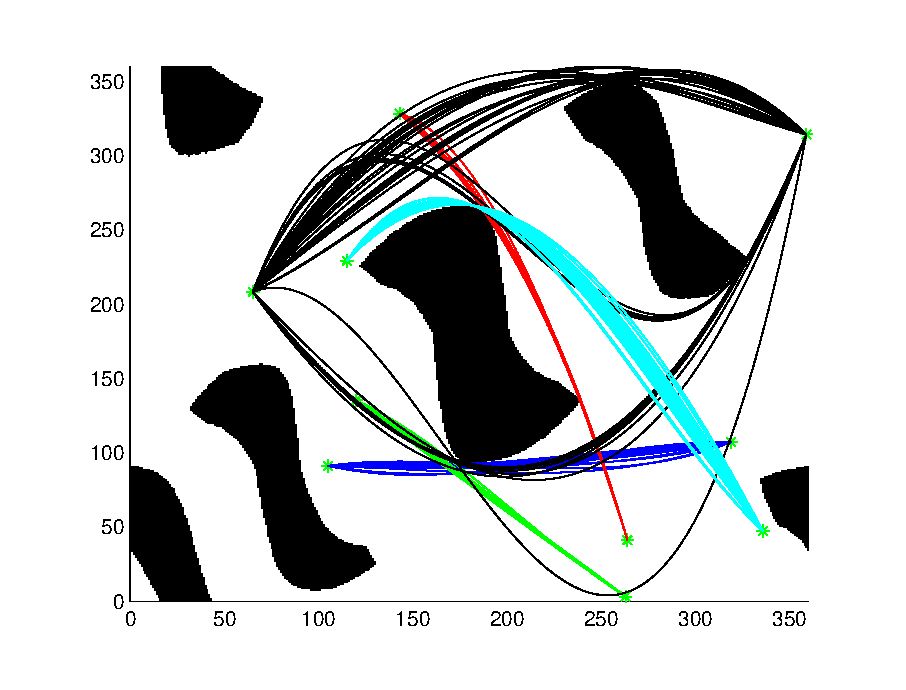
\includegraphics[width=0.55\textwidth]{./figures/results_cSpace4.eps}
	\caption{Resultant optimized paths from 40 trials on five start\/end point sets. Axis represent the full range of motion of joints one and two of the manipulator. The algorithm avoids the black areas which represent obstacle collisions.}
	\label{fig:ws2cs}
\end{figure}

The results of the experiment are presented in table \ref{tbl:results}.
number of trials run: 600

{\renewcommand{\arraystretch}{1.4}
	\begin{center}
		\begin{table}[h]
		\begin{tabular}{ c | c  c  p{2cm} }
		Criteria & Result & Unit & Note \\ \hline
		Path length & 0.7 & \% longer & Compared to wavefront method \\ 
		Freq. of shorter path & 79 & \% & Compared to wavefront method \\ 
		Time to completion & 5.15 & seconds & 20767\% improvement on wavefront method \\ 
		Average number of generations & 12.3 & generations & \\ 
		Freq. of collision free path & 94 & \% &  \\ 
		Jerk improvement & 194 & ${{D}\over{T^3}}$ & Compared to implementation not minimizing jerk.\\ 
		\end{tabular}
		\caption{Results obtained through 600 trials of the path finding algorithm.}
		\end{table}
	\end{center}
}


